% =====================================================================
% Guía del estudiante -- Física 11° -- Trimestre I
% Hilo conductor: De Tales al pararrayos
% Temas (de curriculo/programacion.csv, clases 001-021):
%   notacion, carga, coulomb, campo
% =====================================================================
\documentclass[11pt]{article}
\makeatletter\def\input@path{{../../../../plantillas/estilo/}}\makeatother
\usepackage{mmcantillo}

% ======================== DATOS DE LA GUÍA ============================
\tipodocumento{Guía del estudiante}
\asignatura{Física}
\titulo{Cargas, fuerzas y campos: la electricidad que no se ve}
\grado{11°}
\periodo{I}
\hiloconductor{De Tales al pararrayos}
% ======================================================================
% DBA: naturales grado 11 · DBA 2 — Comprende que la interacción de las cargas en reposo
% genera fuerzas eléctricas y que cuando las cargas están en movimiento genera fuerzas
% magnéticas. (dba/naturales/grados/grado11.tex; en este trimestre se trabaja la primera
% parte: cargas en reposo.)

\begin{document}

\encabezado

% ---------------------------------------------------------------------
% 1. Frase introductoria
% ---------------------------------------------------------------------
% verificado: https://founders.archives.gov/documents/Franklin/01-04-02-0135 — Pennsylvania Gazette, 19 oct. 1752: «and thereby the Sameness of the Electric Matter with that of Lightning compleatly demonstrated»
\frase{Con el fuego eléctrico así obtenido [\ldots] queda completamente demostrada la
identidad de la materia eléctrica con la del rayo.}
{Benjamin Franklin, \emph{Pennsylvania Gazette} (19 de octubre de 1752), trad. propia}

% ---------------------------------------------------------------------
% 2. Introducción
% ---------------------------------------------------------------------
\seccion{Introducción}

Cuando te quitas un saco de lana y escuchas un chisporroteo, cuando el pelo se te pega al
peine, cuando sientes un corrientazo al tocar la puerta de un carro: en todos esos casos
está ocurriendo lo mismo que en un rayo, solo que a una escala millones de veces menor. En
este trimestre vamos a estudiar de dónde salen esas fuerzas, cómo se calculan y por qué
actúan a distancia, sin que nada visible conecte a los objetos.

Nuestro hilo conductor es una historia de 2600 años. Empieza con un filósofo griego que
frota un trozo de ámbar, sigue con un médico inglés que separa dos fenómenos que todo el
mundo confundía, pasa por un ingeniero francés que pesa una fuerza invisible con una
balanza de hilos, y termina con un impresor de Filadelfia que sube una cometa en plena
tormenta y regresa con la idea del pararrayos. En cada tema daremos un paso de esa
historia.

\textbf{Al terminar este trimestre podrás:}
\begin{itemize}
  \item expresar cantidades muy grandes y muy pequeñas en notación científica y comparar
        órdenes de magnitud;
  \item explicar cómo se electriza un cuerpo por frotamiento, contacto e inducción, y
        distinguir conductores de aislantes;
  \item calcular la fuerza eléctrica entre cargas puntuales con la ley de Coulomb y sumar
        las fuerzas de varias cargas;
  \item describir el campo eléctrico de una o varias cargas, dibujar sus líneas y usarlo
        para explicar aplicaciones como el pararrayos.
\end{itemize}

Este trimestre trabaja el siguiente Derecho Básico de Aprendizaje del Ministerio de
Educación Nacional~\cite{mendba}; en el trimestre I nos ocupamos de su primera parte, las
cargas en reposo:

\begin{dba}[Grado 11 · DBA 2]
Comprende que la interacción de las cargas en reposo genera fuerzas eléctricas y que cuando
las cargas están en movimiento genera fuerzas magnéticas.
\end{dba}

También responde a los estándares del grupo de grados 10.º--11.º de Ciencias
Naturales~\cite{menestandares}: establecer relaciones entre fuerzas macroscópicas y fuerzas
electrostáticas, y entre el campo gravitacional y el electrostático.

% ---------------------------------------------------------------------
% 3. Marco teórico
% ---------------------------------------------------------------------
\seccion{Marco teórico}

\subsubsection*{Un trozo de ámbar y una palabra griega}

La primera observación registrada de la electricidad es muy sencilla: al frotar ámbar con
un paño, el ámbar atrae plumas, hilos y trocitos de paja. La tradición griega atribuye esa
observación a Tales de Mileto, en el siglo \textsc{vi} a.\,C. El ámbar se llamaba en griego
\emph{élektron}, y de esa palabra viene todo el vocabulario que usamos hoy: electricidad,
electrón, electrónica.

Durante veintiún siglos no pasó mucho más. En 1600, el médico inglés William Gilbert
publicó \emph{De magnete}~\cite{gilbert1600}, el primer estudio sistemático del magnetismo
y de lo que él llamó los cuerpos \emph{eléctricos}: los que, como el ámbar, atraen objetos
livianos después de ser frotados. Gilbert hizo algo que parece obvio y no lo era: mostró
que la atracción del imán y la atracción del ámbar son fenómenos \emph{distintos}. Hoy
sabemos que están profundamente relacionados ---eso es justamente lo que dice la segunda
parte de nuestro DBA--- pero para entenderlos primero había que separarlos.

\subsubsection*{Medir lo invisible}

En el siglo \textsc{xviii} la electricidad pasó de curiosidad de salón a objeto de medida.
En 1785, el ingeniero militar francés Charles-Augustin de Coulomb presentó a la Academia de
Ciencias un experimento hecho con una balanza de torsión: una aguja colgada de un hilo muy
fino, tan sensible que el giro del hilo permitía medir fuerzas diminutas~\cite{coulomb1785}.
Con ella estableció que la fuerza entre dos cuerpos electrizados disminuye con el cuadrado
de la distancia, igual que la fuerza de gravedad de Newton. Dos fuerzas muy distintas
obedecen la misma forma matemática: esa es una de las razones por las que la física confía
en las matemáticas.

En esos mismos años, la ciencia experimental europea empezaba, muy lentamente, a abrirse a
las mujeres. Laura Bassi se graduó en filosofía en la Universidad de Bolonia en 1732, a los
veinte años, y en 1776 obtuvo la cátedra de física experimental del Instituto de Ciencias
de esa ciudad~\cite{bassi}: fue una de las primeras mujeres de Europa en enseñar física
experimental en una universidad, en la misma época en que Coulomb hacía sus mediciones.

\subsubsection*{Del rayo al pararrayos}

Mientras tanto, en Filadelfia, Benjamin Franklin sostenía una idea arriesgada: que el rayo
no era un castigo divino ni un fenómeno aparte, sino el mismo tipo de electricidad que se
produce frotando vidrio, solo que a una escala enorme. En octubre de 1752 publicó las
instrucciones del experimento de la cometa con una llave~\cite{franklin1752}, y de ahí salió
un invento que todavía protege los edificios de tu ciudad: el pararrayos. La frase con la
que abre esta guía es suya.

El paso final de la historia es una idea que cambió la física: en lugar de pensar que dos
cargas se jalan «a distancia», podemos decir que cada carga modifica el espacio a su
alrededor ---crea un \textbf{campo}--- y que la otra carga responde al campo que hay donde
ella está. Esa manera de verlo, que se formalizó en el siglo \textsc{xix}, es la que
usaremos en el último tema y la que nos llevará, el próximo trimestre, a la corriente y al
magnetismo~\cite{serway2019}.

% ---------------------------------------------------------------------
% 4. Temas
% ---------------------------------------------------------------------
\tema{Notación científica y orden de magnitud}\label{tema:notacion}

\begin{hilo}
Tales frota su ámbar y atrae una pluma. La fuerza que actúa ahí es minúscula, y la cantidad
de carga que se transfiere también: para hablar de ella necesitaríamos escribir
\num{0,000000001} coulomb. Antes de estudiar la electricidad hay que aprender a escribir
los números con los que trabaja.
\end{hilo}

Un número está en \textbf{notación científica} cuando se escribe como $a \times 10^{n}$, con
$1 \le |a| < 10$ y $n$ entero. El \textbf{orden de magnitud} de una cantidad es la potencia
de diez que más se le parece: sirve para comparar sin hacer cuentas exactas.

\begin{ejemplo}[Las constantes de este trimestre]
La carga de un electrón es $e = \num{1,602e-19}$ C; su masa, $m_e = \num{9,11e-31}$ kg; y la
constante eléctrica que usaremos, $k = \num{8,99e9}$ N\,m\textsuperscript{2}/C\textsuperscript{2}.
La carga del electrón es diminuta y $k$ es enorme: escritas sin potencias de diez, la
primera tendría 18 ceros después de la coma y la segunda, diez cifras. Por eso en este
trimestre todo se escribe en notación científica.
\end{ejemplo}

\begin{ejemplo}[Prefijos]
$\qty{1}{\micro\coulomb} = \num{1e-6}$ C, $\qty{1}{\nano\coulomb} = \num{1e-9}$ C,
$\qty{1}{\kilo\newton} = \num{1e3}$ N. Escribir \qty{2,5}{\micro\coulomb} es más cómodo que
escribir \num{0,0000025} C, y es el mismo número.
\end{ejemplo}

\begin{aplicacion}[Por qué a los físicos les importan los órdenes de magnitud]
Antes de resolver un problema, un físico estima. Si vas a calcular la fuerza entre dos
cargas típicas de laboratorio y te da un resultado del orden de \num{e12} N ---más que el
peso de una montaña--- casi seguro te equivocaste en una potencia de diez. La estimación no
reemplaza el cálculo: lo protege.
\end{aplicacion}

\begin{preguntas}
\pregunta Escribe en notación científica: la distancia \qty{0,000045}{m}, la carga
\qty{32000}{\nano\coulomb} expresada en coulomb, y la masa \qty{0,0000000012}{kg}.
\espacio{2.5cm}
\pregunta ¿Cuántos electrones hacen falta para reunir una carga de \qty{1}{\nano\coulomb}?
Escribe el resultado en notación científica.
\espacio{3cm}
\pregunta Un estudiante afirma que $\num{4e-6} + \num{3e-7} = \num{7e-13}$. Encuentra el
error, explícalo con tus palabras y da el resultado correcto.
\renglones{3}
\end{preguntas}

\begin{resumen}
\begin{itemize}
  \item En notación científica todo número se escribe como $a\times 10^{n}$ con
        $1 \le |a| < 10$.
  \item El orden de magnitud es la potencia de diez más cercana: sirve para comparar y para
        detectar errores.
  \item Los prefijos (micro, nano, kilo) son notación científica disfrazada.
\end{itemize}
\end{resumen}

\tema{La carga eléctrica}\label{tema:carga}

\begin{hilo}
Gilbert repite el experimento del ámbar cientos de veces, con azufre, vidrio, resina y
piedras preciosas, y anota cuáles atraen y cuáles no. Está haciendo lo que tú harás en el
laboratorio de este tema: clasificar los materiales según cómo se comportan al frotarlos.
\end{hilo}

\begin{definicion}[Carga eléctrica]
La carga eléctrica es una propiedad de la materia que existe en dos clases, llamadas
\emph{positiva} y \emph{negativa}. Cargas de la misma clase se repelen; cargas de clases
distintas se atraen. Su unidad en el SI es el \textbf{coulomb} (C).
\end{definicion}

Sobre la carga hay dos principios que conviene tener claros desde el comienzo:

\begin{itemize}
  \item \textbf{Conservación:} la carga no se crea ni se destruye. Cuando frotas un globo
        contra tu pelo, no aparece carga nueva: unos electrones \emph{pasan} del pelo al
        globo, y el globo queda negativo justo en la misma medida en que el pelo queda
        positivo.
  \item \textbf{Cuantización:} toda carga es un múltiplo entero de la carga elemental,
        $q = n\,e$ con $e = \num{1,602e-19}$ C. No existe media carga elemental.
\end{itemize}

Un cuerpo se electriza de tres maneras. Por \textbf{frotamiento}, cuando dos materiales
distintos se rozan y uno le arranca electrones al otro. Por \textbf{contacto}, cuando un
cuerpo cargado toca a otro y le comparte parte de su carga: los dos quedan con carga del
mismo signo. Y por \textbf{inducción}, cuando un cuerpo cargado se \emph{acerca} sin tocar y
obliga a las cargas del otro a reacomodarse; si en ese momento el segundo cuerpo se conecta
a tierra, queda cargado con el signo contrario al del inductor.

Los materiales en los que las cargas se mueven con facilidad se llaman \textbf{conductores}
(los metales, el agua con sales, el cuerpo humano); aquellos en los que las cargas se quedan
donde se depositan son \textbf{aislantes} (el vidrio, el plástico, la madera seca, el
caucho).

\begin{ejemplo}[¿Cuántos electrones sobran?]
Un globo frotado adquiere una carga de $\qty{-2}{\nano\coulomb}$. Como
$q = n\,e$, el número de electrones en exceso es
\[
  n = \frac{\num{2e-9}}{\num{1,602e-19}} \approx \num{1,25e10},
\]
es decir, unos doce mil quinientos millones de electrones de más. Parece muchísimo, pero es
una fracción minúscula de los electrones que tiene el globo.
\end{ejemplo}

\begin{aplicacion}[Por qué los camiones de combustible se conectan a tierra]
Al bombear un líquido por una manguera, el roce electriza tanto al líquido como al tubo. Si
esa carga se acumula, puede saltar una chispa, y junto a vapores de gasolina una chispa es
un incendio. Por eso los camiones cisterna se conectan a tierra antes de descargar: la
conexión da a las cargas un camino conductor para irse, en lugar de acumularse. Es el mismo
principio de la pulsera antiestática que usa un técnico al manipular la tarjeta de un
computador.
\end{aplicacion}

\begin{preguntas}
\pregunta Explica, usando la conservación de la carga, por qué después de frotar un globo
contra tu pelo el globo y el pelo quedan con cargas de signos opuestos y de igual magnitud.
\renglones{3}
\pregunta Una barra cargada positivamente se acerca ---sin tocar--- a una esfera metálica
descargada y aislada. Describe cómo quedan distribuidas las cargas en la esfera y explica por
qué la esfera es atraída, aunque su carga total siga siendo cero.
\renglones{4}
\pregunta Un compañero dice: «como el cuerpo humano es conductor, tocar un objeto cargado
siempre nos electriza». Discute la afirmación: ¿en qué caso el cuerpo se carga y en cuál no?
\renglones{3}
\pregunta Calcula la carga total de $\num{5e12}$ electrones y exprésala en nanocoulomb, con su
signo.
\espacio{2.5cm}
\end{preguntas}

\begin{resumen}
\begin{itemize}
  \item Hay dos clases de carga; las iguales se repelen y las distintas se atraen.
  \item La carga se conserva y está cuantizada: $q = n\,e$, con $e=\num{1,602e-19}$ C.
  \item Un cuerpo se electriza por frotamiento, por contacto o por inducción.
  \item En los conductores las cargas se mueven con facilidad; en los aislantes, no.
\end{itemize}
\end{resumen}

\tema{La ley de Coulomb}\label{tema:coulomb}

\begin{hilo}
Coulomb cuelga una aguja de un hilo de plata finísimo dentro de un cilindro de vidrio, para
que ni una corriente de aire perturbe la medida. Carga dos esferitas, las acerca y mide
cuánto gira el hilo. Está a punto de convertir una curiosidad en una ley con números.
\end{hilo}

\begin{definicion}[Ley de Coulomb]
La fuerza eléctrica entre dos cargas puntuales $q_1$ y $q_2$ separadas una distancia $r$
tiene magnitud
\[
  F = k\,\frac{|q_1 q_2|}{r^{2}}, \qquad k = \num{8,99e9}\ \mathrm{N\,m^{2}/C^{2}},
\]
está dirigida a lo largo de la recta que une las cargas, y es de repulsión si las cargas
tienen el mismo signo y de atracción si tienen signos contrarios.
\end{definicion}

Dos consecuencias que conviene tener presentes. La primera: la fuerza depende del
\emph{cuadrado} de la distancia, así que si alejas las cargas al doble, la fuerza no se
reduce a la mitad sino a la cuarta parte. La segunda: cuando hay más de dos cargas, la
fuerza sobre una de ellas es la \textbf{suma vectorial} de las fuerzas que cada una de las
otras ejerce por separado. A eso se le llama principio de superposición.

\begin{ejemplo}[Dos cargas puntuales]
Sean $q_1 = \qty{2}{\micro\coulomb}$ y $q_2 = \qty{-3}{\micro\coulomb}$, separadas
$r = \qty{5}{cm} = \qty{0,05}{m}$:
\[
  F = \num{8,99e9}\cdot\frac{(\num{2e-6})(\num{3e-6})}{(\num{0,05})^{2}}
    = \frac{\num{5,394e-2}}{\num{2,5e-3}} \approx \qty{21,6}{N}.
\]
Como los signos son contrarios, la fuerza es de atracción, y por la tercera ley de Newton
cada carga siente \qty{21,6}{N} hacia la otra.
\end{ejemplo}

\begin{ejemplo}[Eléctrica contra gravitacional]
Entre dos electrones actúan las dos fuerzas a la vez. Su cociente no depende de la
distancia, porque ambas van como $1/r^{2}$:
\[
  \frac{F_e}{F_g} = \frac{k\,e^{2}}{G\,m_e^{2}} \approx \num{4e42}.
\]
La fuerza eléctrica es unas $\num{e42}$ veces más intensa. Si es tan fuerte, ¿por qué no la
notamos todo el tiempo? Porque la materia ordinaria tiene tantas cargas positivas como
negativas y sus efectos se cancelan; la gravedad, en cambio, solo atrae y nunca se cancela.
\end{ejemplo}

\begin{aplicacion}[Pintar un carro sin desperdiciar pintura]
En las plantas automotrices la pintura se pulveriza cargada eléctricamente y la carrocería
se conecta con carga contraria. Las gotas son atraídas hacia la lámina, se reparten parejo
e incluso rodean los bordes, en vez de perderse en el aire. La misma idea está detrás de las
impresoras láser, donde el tóner cargado se adhiere solo a las zonas del rodillo que llevan
carga contraria.
\end{aplicacion}

\begin{preguntas}
\pregunta Dos cargas iguales de \qty{4}{\micro\coulomb} están separadas \qty{10}{cm}.
Calcula la fuerza entre ellas e indica si es de atracción o de repulsión.
\espacio{3cm}
\pregunta Si en el ejercicio anterior la distancia se triplica, ¿por qué factor cambia la
fuerza? Responde primero razonando, sin calculadora, y después compruébalo con el cálculo.
\espacio{3cm}
\pregunta Tres cargas están sobre una misma línea: $q_1=\qty{+2}{\micro\coulomb}$ en
$x=0$, $q_2=\qty{-2}{\micro\coulomb}$ en $x=\qty{20}{cm}$ y $q_3=\qty{+1}{\micro\coulomb}$
en $x=\qty{40}{cm}$. Calcula la fuerza neta sobre $q_3$ (magnitud y sentido).
\espacio{4cm}
\pregunta Un estudiante calcula la fuerza entre dos cargas separadas \qty{20}{cm} y escribe
$r^2 = \num{400}$. Encuentra el error y explica qué consecuencia tiene en el resultado.
\renglones{3}
\end{preguntas}

\begin{resumen}
\begin{itemize}
  \item $F = k\,|q_1q_2|/r^{2}$, con $k=\num{8,99e9}$ N\,m\textsuperscript{2}/C\textsuperscript{2}
        y la distancia \emph{siempre} en metros.
  \item Al duplicar la distancia la fuerza se reduce a la cuarta parte: es una ley del
        inverso del cuadrado.
  \item Con varias cargas, las fuerzas se suman como vectores (superposición).
  \item La fuerza eléctrica puede atraer o repeler; la gravitacional solo atrae.
\end{itemize}
\end{resumen}

\tema{El campo eléctrico}\label{tema:campo}

\begin{hilo}
Franklin sube una cometa en medio de una tormenta y consigue cargar una botella de Leyden
desde una llave atada al cordel. El rayo y la chispa del laboratorio son lo mismo. Pero
queda una pregunta incómoda: si nada toca a la carga, ¿\emph{cómo} le llega la fuerza?
\end{hilo}

\begin{definicion}[Campo eléctrico]
El campo eléctrico en un punto es la fuerza por unidad de carga que sentiría allí una carga
de prueba positiva $q_0$:
\[
  \vect{E} = \frac{\vect{F}}{q_0}, \qquad [E] = \mathrm{N/C}.
\]
Para una carga puntual $q$ a una distancia $r$, su magnitud es $E = k\,|q|/r^{2}$, y apunta
alejándose de la carga si $q>0$ y hacia la carga si $q<0$.
\end{definicion}

El campo se dibuja con \textbf{líneas de campo}: salen de las cargas positivas y entran a
las negativas, nunca se cruzan, y son más densas donde el campo es más intenso. La fuerza
sobre una carga positiva colocada en el campo va en el sentido de la línea; sobre una carga
negativa, en el sentido contrario.

\begin{center}
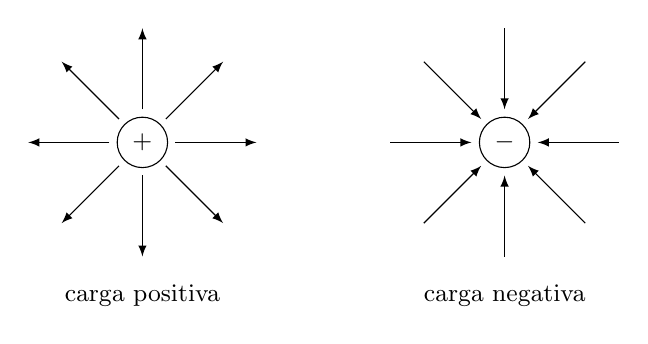
\begin{tikzpicture}[scale=1, >=latex, font=\small]
  % carga positiva
  \begin{scope}
    \foreach \a in {0,45,...,315}
      \draw[->] (\a:0.42) -- (\a:1.45);
    \draw[fill=white] (0,0) circle (0.32);
    \node at (0,0) {$+$};
    \node at (0,-1.95) {carga positiva};
  \end{scope}
  % carga negativa
  \begin{scope}[xshift=4.6cm]
    \foreach \a in {0,45,...,315}
      \draw[<-] (\a:0.42) -- (\a:1.45);
    \draw[fill=white] (0,0) circle (0.32);
    \node at (0,0) {$-$};
    \node at (0,-1.95) {carga negativa};
  \end{scope}
\end{tikzpicture}
\end{center}

\begin{ejemplo}[Campo de una carga puntual]
A \qty{30}{cm} de una carga de \qty{5}{\micro\coulomb}:
\[
  E = \num{8,99e9}\cdot\frac{\num{5e-6}}{(\num{0,30})^{2}}
    = \frac{\num{4,495e4}}{\num{9e-2}} \approx \num{5,0e5}\ \mathrm{N/C},
\]
dirigido alejándose de la carga. Una carga de prueba de \qty{2}{\nano\coulomb} colocada allí
sentiría $F = qE = \num{2e-9}\cdot\num{5,0e5} \approx \qty{1,0e-3}{N}$.
\end{ejemplo}

\begin{aplicacion}[El pararrayos y la jaula de Faraday]
En las puntas afiladas de un conductor el campo eléctrico se hace mucho más intenso que en
las superficies planas. El pararrayos aprovecha eso: su punta ioniza el aire a su alrededor y
ofrece al rayo un camino conductor hasta tierra, lejos de la estructura del edificio. El
fenómeno complementario también se usa: dentro de una caja metálica cerrada el campo externo
no penetra, y por eso un carro o un avión son lugares relativamente seguros durante una
tormenta eléctrica. A esa protección se le llama jaula de Faraday~\cite{serway2019}.
\end{aplicacion}

\begin{preguntas}
\pregunta Calcula la magnitud del campo eléctrico a \qty{15}{cm} de una carga de
\qty{-3}{\micro\coulomb} e indica hacia dónde apunta.
\espacio{3cm}
\pregunta En un punto donde el campo vale \qty{2,0e4}{N/C} se coloca una carga de
\qty{-5}{\nano\coulomb}. Calcula la magnitud de la fuerza y explica por qué su sentido es
opuesto al del campo.
\espacio{3cm}
\pregunta Dibuja las líneas de campo de dos cargas iguales y positivas, y señala un punto
donde el campo total sea cero. Justifica por qué lo es.
\espacio{4cm}
\pregunta Explica por qué las líneas de campo no pueden cruzarse. (Pista: ¿qué significaría,
para la fuerza sobre una carga de prueba, que dos líneas pasaran por el mismo punto?)
\renglones{3}
\end{preguntas}

\begin{resumen}
\begin{itemize}
  \item $\vect{E} = \vect{F}/q_0$, y para una carga puntual $E = k|q|/r^{2}$, en N/C.
  \item Las líneas salen de lo positivo y entran a lo negativo; no se cruzan y su densidad
        indica la intensidad del campo.
  \item Sobre una carga negativa la fuerza es opuesta al campo.
  \item El campo se concentra en las puntas (pararrayos) y no entra en el interior de un
        conductor cerrado (jaula de Faraday).
\end{itemize}
\end{resumen}

% ---------------------------------------------------------------------
% 5. Saber 11
% ---------------------------------------------------------------------
\seccion{Prepárate para Saber 11}

\begin{preguntas}
\pregunta La carga de un electrón es $\num{1,602e-19}$ C. La carga de un cuerpo que tiene
$\num{2,0e13}$ electrones en exceso es, aproximadamente:
\begin{opciones*}(4)
  \item \qty{3,2}{\micro\coulomb}
  \item \qty{-3,2}{\micro\coulomb}
  \item \qty{3,2}{\nano\coulomb}
  \item \qty{-3,2}{\nano\coulomb}
\end{opciones*}

\pregunta Dos esferas con cargas iguales se repelen con una fuerza $F$ cuando están separadas
una distancia $d$. Si la separación se reduce a $d/2$, la fuerza entre ellas será:
\begin{opciones*}(4)
  \item $F/4$
  \item $F/2$
  \item $2F$
  \item $4F$
\end{opciones*}

\pregunta Una barra cargada negativamente se acerca, sin tocarla, a una esfera metálica
neutra y aislada. Lo que ocurre en la esfera es que:
\begin{opciones*}(2)
  \item gana electrones y queda cargada negativamente
  \item pierde protones y queda cargada negativamente
  \item sus electrones se alejan de la barra y la cara cercana queda positiva
  \item no ocurre nada, porque la barra no la toca
\end{opciones*}

\pregunta En una región el campo eléctrico apunta hacia la derecha. Si allí se coloca una
carga negativa, la fuerza eléctrica sobre ella:
\begin{opciones*}(2)
  \item apunta hacia la derecha y es proporcional al campo
  \item apunta hacia la izquierda y es proporcional al campo
  \item es cero, porque la carga es negativa
  \item apunta hacia la derecha, pero no depende del valor de la carga
\end{opciones*}
\end{preguntas}

% ---------------------------------------------------------------------
% 6. Cierre del hilo conductor
% ---------------------------------------------------------------------
\seccion{Cierre: del ámbar al pararrayos}

Empezamos con un filósofo frotando una piedra amarilla y terminamos con una varilla metálica
que protege un edificio de un rayo de millones de voltios. En el camino, Gilbert separó dos
fenómenos que parecían uno solo, Coulomb midió con un hilo de plata una fuerza que nadie
podía ver, y Franklin se atrevió a proponer que el rayo del cielo y la chispa del laboratorio
eran la misma cosa.

Queda una pregunta abierta, y es la que abre el próximo trimestre. Todo lo que estudiamos
aquí ocurre con las cargas \emph{quietas}. ¿Qué pasa cuando las ponemos a moverse? Aparecen
la corriente, los circuitos y algo que Gilbert había separado con tanto cuidado: el
magnetismo, que resulta estar íntimamente ligado a la electricidad. Esa es la segunda parte
de nuestro DBA, y la veremos en el trimestre II.

% ---------------------------------------------------------------------
% 7. Evaluación
% ---------------------------------------------------------------------
\matrizevaluacion
  {Explica la naturaleza de la carga eléctrica, las formas de electrización y el concepto de campo.}
  {Calcula fuerzas y campos eléctricos con la ley de Coulomb y el principio de superposición, con unidades correctas.}
  {Estima órdenes de magnitud y revisa sus resultados antes de darlos por buenos.}
  {Trabaja en equipo en el laboratorio y cuida los materiales y a sus compañeros.}

\autoevaluacion

\seguimientodocente

% ---------------------------------------------------------------------
% 8. Referencias
% ---------------------------------------------------------------------
\begin{referencias}
% verificado: https://www.academie-sciences.fr/pdf/dossiers/Coulomb/Coulomb_pdf/Mem1785_p569.pdf — Histoire de l'Académie Royale des Sciences (1785), pp. 569-577, facsímil de la Académie des sciences
\bibitem{coulomb1785} Coulomb, C.-A. (1785). Premier mémoire sur l'électricité et le
  magnétisme. \emph{Histoire de l'Académie Royale des Sciences}, 569--577.
% verificado: https://founders.archives.gov/documents/Franklin/01-04-02-0135 — Founders Online (National Archives): texto publicado en la Pennsylvania Gazette del 19 de octubre de 1752
\bibitem{franklin1752} Franklin, B. (1752, 19 de octubre). [Experimento de la cometa].
  \emph{Pennsylvania Gazette}.
% verificado: https://archive.org/details/1600-william-gilbert-de-magnete — facsímil de la edición de Londres, Peter Short, 1600
\bibitem{gilbert1600} Gilbert, W. (1600). \emph{De magnete, magneticisque corporibus, et de
  magno magnete tellure}. Londres: Peter Short.
% verificado: https://www.mineducacion.gov.co/1780/articles-81033_archivo_pdf.pdf — MEN, Guía n.º 7 (2004), estándares de Ciencias Naturales, grupo 10.º-11.º en la p. 23
\bibitem{menestandares} Ministerio de Educación Nacional (2004). \emph{Formar en ciencias:
  ¡el desafío! Estándares Básicos de Competencias en Ciencias Naturales y Ciencias Sociales}
  (Guía n.º 7). Bogotá: MEN.
% verificado: https://www.colombiaaprende.edu.co/sites/default/files/files_public/2022-06/DBA_C.Naturales-min.pdf — PDF oficial del MEN publicado en Colombia Aprende
\bibitem{mendba} Ministerio de Educación Nacional (2016). \emph{Derechos Básicos de
  Aprendizaje V.1: Ciencias Naturales}. Bogotá: MEN.
% verificado: https://cengagelatam.editorialdc.com/libros/fisica-para-ciencias-e-ingenieria-vol-2/ — ficha de la editorial Cengage para el volumen 2 (electricidad y magnetismo)
\bibitem{serway2019} Serway, R. A. y Jewett, J. W. \emph{Física para ciencias e ingeniería,
  volumen 2}. México: Cengage Learning.
% verificado: https://www.unibo.it/en/university/who-we-are/our-history/famous-people-and-students/laura-bassi — Universidad de Bolonia: nació en 1711, se graduó en filosofía en abril de 1732 y en 1776 obtuvo la cátedra de física experimental del Istituto delle Scienze
\bibitem{bassi} Università di Bologna. \emph{Laura Bassi}. Consultado el 14 de septiembre de 2026.
\end{referencias}

\end{document}
